% Foliensatz: "AFu-Kurs nach DJ4UF" von DK0TU, Amateurfunkgruppe der TU Berlin
% Lizenz: CC BY-NC-SA 3.0 de (http://creativecommons.org/licenses/by-nc-sa/3.0/de/)
% Autoren: 
% Martin Deutschmann
% Lars Weiler <dc4lw@darc.de>

\documentclass[aspectratio=169]{beamer}

\usepackage[ngerman]{babel} % deutsche Worttrennung etc.
\usepackage[utf8]{inputenc} % UTF8 Text

\usepackage[super, comma, numbers, square, sort]{natbib}

\usepackage{hyperref}       % Hyperref Package für bessere Referenzen (todo)
\hypersetup{
	colorlinks=false,       %   false: boxed links; true: colored links
    %linkcolor=white,       %   color of internal links (change box color with linkbordercolor)
    citecolor=red,          %   color of links to bibliography
    filecolor=white,        %   color of file links
    urlcolor=blue           %   color of external links
}

\usepackage{multirow}
\usepackage{wasysym}  % Math Symbols like \permil
%\usepackage{colortbl}
%\usepackage{subscript}
%\usepackage{caption}
%\usepackage{setspace}
%\usepackage{xcolor}        % benutze CodeListe

% Footnote
%\usepackage{hanging}
%
%\setbeamertemplate{footnote}{%
%  \hangpara{2em}{1}%
%  \makebox[2em][l]{\insertfootnotemark}\footnotesize\insertfootnotetext\par%
%}


%\usepackage{pgf}
%\usepackage{tikz}
%\usetikzlibrary{arrows,automata}
%\usetikzlibrary{positioning}
%
%\tikzset{
%    state/.style={
%           rectangle,
%           rounded corners,
%           draw=black, very thick,
%           minimum height=2em,
%           minimum width=2pt,
%           inner sep=2pt,
%           text centered,
%           },
%}

%\usepackage{listings}
%\lstset{basicstyle=\small, numberstyle=\tiny, extendedchars=true, numbers=left, numbersep=5pt}
%\lstset{showtabs=false, showspaces=false, showstringspaces=false}
%%\lstset{backgroundcolor=\color{white!75!lightgray}, , frame=single}
%%\lstset{backgroundcolor=\color{white}}
%%\lstset{backgroundcolor=none}
%\lstset{keywordstyle=\color{blue!50!gray},  identifierstyle=\color{black}}
%\lstset{commentstyle=\color{green!50!gray}, stringstyle=\color{red!50!gray}}
%\lstset{language=C, fontadjust=true, tabsize=2, breaklines=true}
%\lstset{backgroundcolor=\color{white!75!lightgray}, caption=\lstname, frame=single}
%\lstset{emphstyle=\color{black}\fbox}
%
%% Keine "Listing:"-Caption
%\captionsetup{labelformat=empty,labelsep=none}
%
%% für mathematische Umgebungen
%\usepackage{amsmath,amsfonts,amssymb}
%
%\lstdefinestyle{Bash}{
%language=Bash,
%frame=single,
%rulecolor=\color{black},
%backgroundcolor=\color{gray!50},
%keywordstyle=\color{black},
%identifierstyle=,
%commentstyle=\color{black},
%stringstyle=\color{magenta!65!white},
%showstringspaces=false,
%basicstyle=\footnotesize\ttfamily\color{black},
%numbers=none,
%breaklines=true,
%captionpos=b
%}

%\usepackage{listings}
%
%\lstdefinestyle{basic}{
%    captionpos=t,%
%    basicstyle=\footnotesize\ttfamily,%
%    numberstyle=\tiny,%
%    numbers=left,%
%    stepnumber=1,%
%    frame=single,%
%    showspaces=false,%
%    showstringspaces=false,%
%    showtabs=false,%
%    %
%    keywordstyle=\color{blue},%
%    identifierstyle=,%
%    commentstyle=\color{gray},%
%    stringstyle=\color{magenta}%
%}



% fließende Boxen haben keinen Abstand
%\fboxsep0mm

% inkludiere Creative Commons Helper
%%%%%%%%%%%%%%%%%%%%%%%%%%%%%%%%%%%%%%%%%%%%%%%%%%%%%%%%%%%%%%%%
%% ccBeamer 0.1, 2007-07-02                                   %%
%% Written by Sebastian Pipping <webmaster@hartwork.org>      %%
%% ---------------------------------------------------------- %%
%% Licensed under Creative Commons Attribution-ShareAlike 3.0 %%
%% http://creativecommons.org/licenses/by-sa/3.0/             %%
%%%%%%%%%%%%%%%%%%%%%%%%%%%%%%%%%%%%%%%%%%%%%%%%%%%%%%%%%%%%%%%%


%% Images
\newcommand{\CcImageBy}[1]{%
	
\includegraphics[scale=#1]{texdata/creative_commons/cc_by_30.pdf}%
}
\newcommand{\CcImageCc}[1]{%
	
\includegraphics[scale=#1]{texdata/creative_commons/cc_cc_30.pdf}%
}
\newcommand{\CcImageDevNations}[1]{%
	
\includegraphics[scale=#1]{texdata/creative_commons/cc_dev_nations_30.pdf}%
}
\newcommand{\CcImageNc}[1]{%
	
\includegraphics[scale=#1]{texdata/creative_commons/cc_nc_30.pdf}%
}
\newcommand{\CcImageNd}[1]{%
	
\includegraphics[scale=#1]{texdata/creative_commons/cc_nd_30.pdf}%
}
\newcommand{\CcImagePd}[1]{%
	
\includegraphics[scale=#1]{texdata/creative_commons/cc_pd_30.pdf}%
}
\newcommand{\CcImageSa}[1]{%
	
\includegraphics[scale=#1]{texdata/creative_commons/cc_sa_30.pdf}%
}
\newcommand{\CcImageSampling}[1]{%
	
\includegraphics[scale=#1]{texdata/creative_commons/cc_sampling_30.pdf}%
}
\newcommand{\CcImageSamplingPlus}[1]{%
	
\includegraphics[scale=#1]{texdata/creative_commons/cc_sampling_plus_30.pdf}%
}


%% Groups
\newcommand{\CcGroupBy}[2]{% zoom, gap
	\CcImageCc{#1}\hspace*{#2}\CcImageBy{#1}%
}
\newcommand{\CcGroupByNc}[2]{% zoom, gap
	\CcImageCc{#1}\hspace*{#2}\CcImageBy{#1}\hspace*{#2}\CcImageNc{#1}%
}
\newcommand{\CcGroupByNcNd}[2]{% zoom, gap
	\CcImageCc{#1}\hspace*{#2}\CcImageBy{#1}\hspace*{#2}\CcImageNc{#1}\hspace*{#2}\CcImageNd{#1}%
}
\newcommand{\CcGroupByNcSa}[2]{% zoom, gap
	\CcImageCc{#1}\hspace*{#2}\CcImageBy{#1}\hspace*{#2}\CcImageNc{#1}\hspace*{#2}\CcImageSa{#1}%
}
\newcommand{\CcGroupByNd}[2]{% zoom, gap
	\CcImageCc{#1}\hspace*{#2}\CcImageBy{#1}\hspace*{#2}\CcImageNd{#1}%
}
\newcommand{\CcGroupBySa}[2]{% zoom, gap
	\CcImageCc{#1}\hspace*{#2}\CcImageBy{#1}\hspace*{#2}\CcImageSa{#1}%
}
\newcommand{\CcGroupDevNations}[2]{% zoom, gap
	\CcImageCc{#1}\hspace*{#2}\CcImageDevNations{#1}%
}
\newcommand{\CcGroupNcSampling}[2]{% zoom, gap
	\CcImageCc{#1}\hspace*{#2}\CcImageNc{#1}\hspace*{#2}\CcImageSampling{#1}%
}
\newcommand{\CcGroupPd}[1]{% zoom
	\CcImagePd{#1}%
}
\newcommand{\CcGroupSampling}[1]{% zoom
	\CcImageSampling{#1}%
}
\newcommand{\CcGroupSamplingPlus}[1]{% zoom
	\CcImageSamplingPlus{#1}%
}


%% Text
\newcommand{\CcLongnameBy}{Attribution}
\newcommand{\CcLongnameByNc}{Attribution-NonCommercial}
\newcommand{\CcLongnameByNcNd}{Attribution-NoDerivs}
\newcommand{\CcLongnameByNcSa}{Attribution-NonCommercial-ShareAlike}
\newcommand{\CcLongnameByNd}{Attribution-NoDerivs}
\newcommand{\CcLongnameBySa}{Attribution-ShareAlike}

\newcommand{\CcNote}[1]{% longname
	This work is licensed under the \textit{Creative Commons #1 3.0 License}.%
}


% generelles Thema auswählen
\usetheme{Goettingen} %Berlin spart ohne Sidebar allerdings angenehm Platz
% AnnArbor | Antibes | Bergen | Berkeley | Berlin | Boadilla | boxes | CambridgeUS | Copenhagen | Darmstadt | default | Dresden | Frankfurt | Goettingen | Hannover | Ilmenau | JuanLesPins | Luebeck | Madrid | Malmoe | Marburg | Montpellier | PaloAlto | Pittsburgh | Rochester | Singapore | Szeged | Warsaw

% Farben wählen
\usecolortheme{beetle}
% beaver | beetle | crane | default | dolphin | dove | fly | lily | orchid | rose | seagull | seahorse | sidebartab | structure | whale | wolverine

% Setze alle Farben auf Grau und Weiß
%\definecolor{craneorange}{RGB}{64,64,64}
%\definecolor{craneblue}{RGB}{255,255,255}

% Schriftart wählen
\usefonttheme{default}
% default | professionalfonts | serif | structurebold | structureitalicserif | structuresmallcapsserif

% Innere Themen(Kopf-, Fuß-, Sidebar usw)
%\useinnertheme{default}
\useinnertheme{circles}
% default | inmargin | rectangles | rounded | circles

% Äußere Themen (Anordnung der inneren, grenzen der Folien etc.)
\useoutertheme{infolines}
% default | infolines | miniframes | shadow | sidebar | smoothbars | smoothtree | split | tree

% Deaktiviere Navigations-Symbole ({} -> leer)
\setbeamertemplate{navigation symbols}{}
%\setbeamertemplate{navigation symbols}{\large \ifnum \insertframenumber <10 0\fi\insertframenumber/\inserttotalframenumber\vspace*{0.2ex}}

% Zeige ein Hintergrundbild
\setbeamertemplate{background canvas}{
        \hspace*{-2.0cm}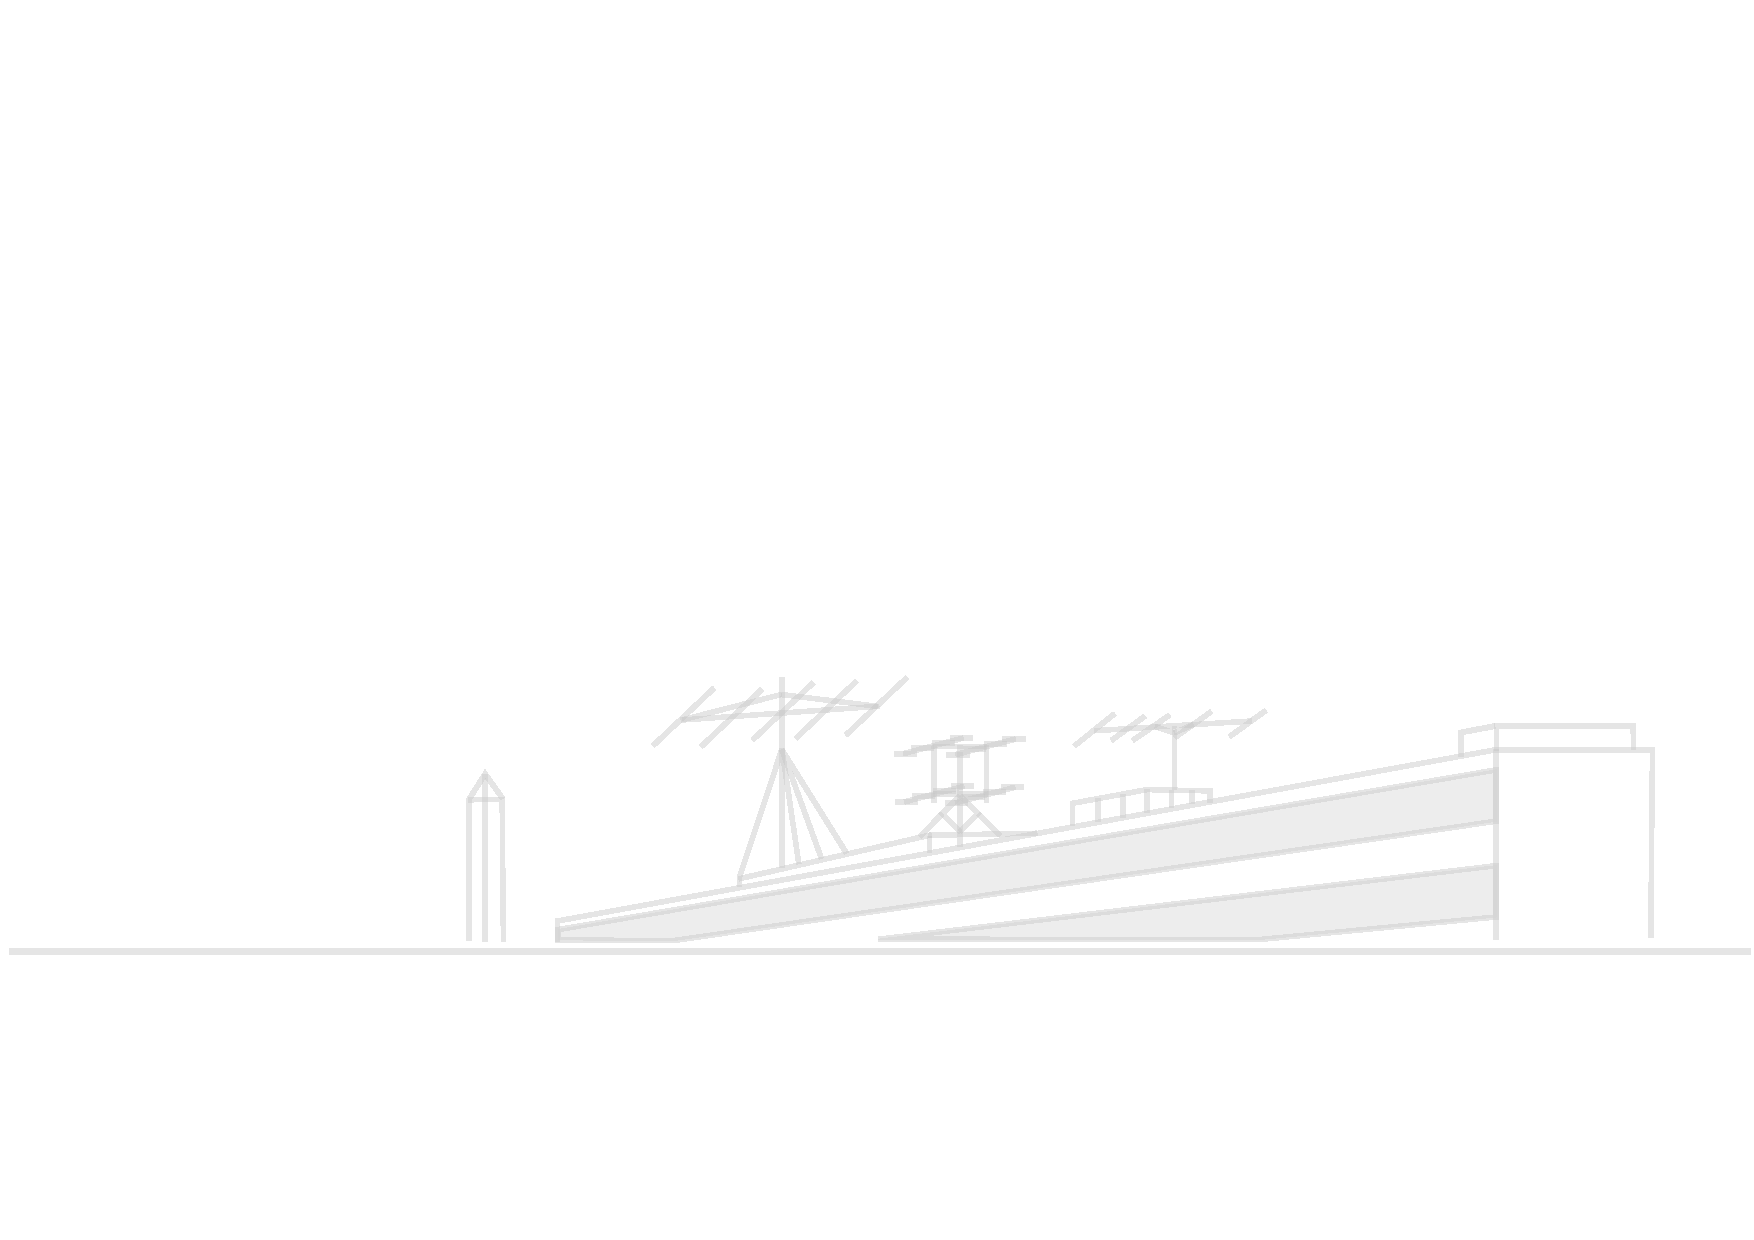
\includegraphics[width=17.8cm]{texdata/dk0tu_rooftop_background.pdf}
}

% Foliennummer einfügen
\setbeamertemplate{footline}[frame number]
%\setbeamertemplate{footline}{}

% Ändere das Zeichen vor jedem item
%\setbeamertemplate{itemize item}{\color{craneorange}$\blacktriangleright$}
%\setbeamertemplate{itemize subitem}{\color{craneorange}$\triangleright$}
%\setbeamertemplate{itemize subsubitem}{\color{craneorange}$\blacktriangleright$}

% Ändert die Blöcke 
\setbeamertemplate{blocks}[rounded][shadow=true]
% default | rounded [shadow=true|false]

%
% Eigene Kommandos
%

% Hack to get natbib and beamer working together. "The beamer user guide suggests
% that only the manual bibliography entry approach is supported"
% on some system it works out of the box, sometimes you need the hack :-(
% so check it --dl7bst
\ifdefined\newblock
    \relax
\else
    \newcommand{\newblock}{}
\fi

% \includedia command to generate png out of a dia file
% NEEDS installed dia and pdflatex option --shell-escape
\newcommand{\includedia}[1]{
    \immediate\write18{/usr/bin/dia #1.dia -e #1_diatmp.png -t png}
}

% RICHIG GROSSER FONT!
\newfont{\bigfont}{cmr10 at 144pt}
\newfont{\smallfont}{cmr10 at 8pt}

% Römische Ziffern
\makeatletter
\newcommand{\rmnum}[1]{\romannumeral #1}
\newcommand{\Rmnum}[1]{\expandafter\@slowromancap\romannumeral #1@}
\makeatother

% Schwarze Überschrift
%\setbeamercolor{frametitle}{fg=black}
%\setbeamercolor{title}{fg=black}

% Item- und Box-Farben
\definecolor{deepBlue}{HTML}{000066}
\setbeamercolor{itemize item}{fg=deepBlue}
\setbeamercolor{itemize subitem}{fg=deepBlue}
\setbeamercolor{description item}{fg=deepBlue}
\setbeamercolor{block title}{fg=deepBlue!100, bg=blue!15}
\setbeamercolor{block body}{fg=black, bg=blue!5}
\setbeamercolor{block title alerted}{fg=deepBlue, bg=red!75}
\setbeamercolor{block body alerted}{fg=black, bg=red!15}
\setbeamercolor*{block title example}{fg=blue!50, bg=blue!10}
\setbeamercolor*{block body example}{fg= blue, bg=blue!5}

%\setbeamercolor{section in head/foot}{parent=palette primary}
%\setbeamercolor{subsection in head/foot}{parent=palette secondary}
%\setbeamercolor{sidebar}{fg=darkblue,bg=yellow!90!orange}
%\setbeamercolor{title in sidebar}{fg=darkblue}
%\setbeamercolor{author in sidebar}{fg=darkblue}
%\setbeamercolor{section in sidebar}{fg=darkblue!10!black}
%\setbeamercolor{subsection in sidebar}{fg=darkblue!50!black}

% Titlepage Infos
\title{AFu-Kurs nach DJ4UF}
\author[DKØTU]{DKØTU\\ \footnotesize{Amateurfunkgruppe der TU Berlin}}
\institute[DKØTU]{\url{http://www.dk0tu.de} }

% PDF-Eigenschaften
\subject{DK0TU-Amateurfunkkurs nach DJ4UF}
\keywords{Amateurfunk Kurs HAM Radio Course CC-BY-NC-SA OpenSource TU Berlin DK0TU}

\subtitle{Technik Klasse A 04: \\
          Schwingkreise \& Filter \\[2em]}
\date{Stand 11.01.2016}
 \begin{document}

\begin{frame}
    \titlepage
    \vfill
    \begin{center}
        \ccbyncsaeu\\
        {\tiny This work is licensed under the \em{Creative Commons Attribution-NonCommercial-ShareAlike 3.0 License}.}\\[0.5ex]
         \tiny Amateurfunkgruppe der Technische Universität Berlin (AfuTUB), DKØTU
         %\includegraphics[scale=0.5]{img/DK0TU_Logo.pdf}
    \end{center}
\end{frame}


%fixme Links zur bibliography einfuegen

\section*{Schwingkreis}
\begin{frame}
\frametitle{Schwingkreise}
	\begin{center}
		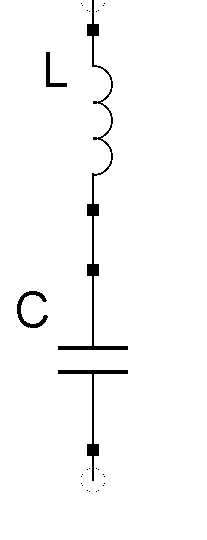
\includegraphics[scale=0.4]{a04/Schwingkreis_reihe.png}
		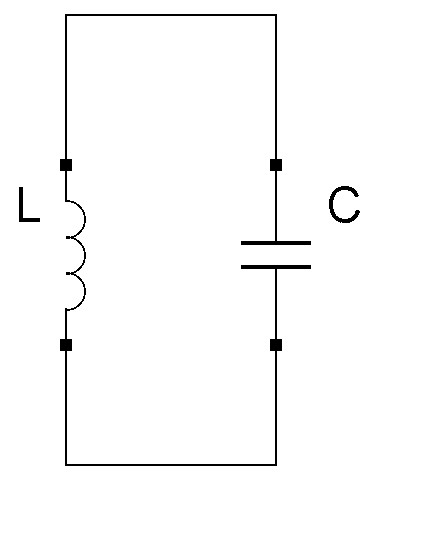
\includegraphics[scale=0.4]{a04/Schwingkreis_parallel.png}\\
		Abb.1: Serien- \& Parallelschwingkreis
	\end{center}
\end{frame}

\begin{frame}
\frametitle{Schwingungserzeugung}
\begin{center}
	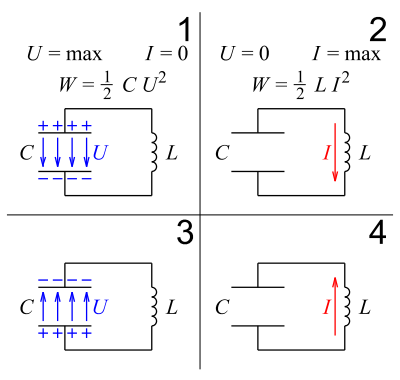
\includegraphics[scale=0.35]{a04/Schwingkreis.png}\\
	{\tiny Abb.2: Energie in einem LC-Schwingkreis \cite{wmde}} \\
	\vspace{3mm}
	\begin{itemize}
		\item durch Verluste kommt es zur gedämpfte Schwingung\\
		\item animierte Darstellung (\url{http://en.wikipedia.org/wiki/File:Tuned_circuit_animation_3.gif})
	\end{itemize}
\end{center}
\end{frame}

\subsection*{Reihen\-schwing\-kreis}
\begin{frame}
\frametitle{Reihenschwingkreis}
\begin{center}
	\begin{minipage}{0.4\textwidth}
	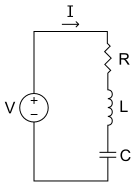
\includegraphics[height=.5\textheight,width=\textwidth,keepaspectratio]{a04/Serirenschw.png}\\
	\tiny{Abb.3: Serienschwingkreis \cite{wmen}}
	\end{minipage}
	\begin{minipage}{0.4\textwidth}
	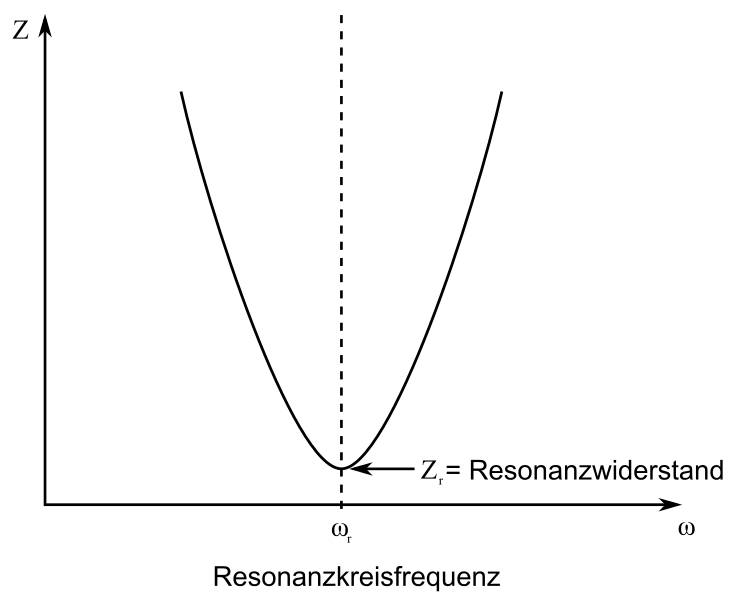
\includegraphics[height=.5\textheight,width=\textwidth,keepaspectratio]{a04/SerirenschwSig.png}\\
	\tiny{Abb.4: Resonanzwiderstand \cite{wmen}} 
	\end{minipage}
\end{center}
\begin{itemize}
	\item Im Verlauf der Frequenzänderung ändert sich der Gesamtwellenwiderstand Z des Schwingkreises
	\item Der Schwingkreis hat als minimale Impedanz seinen ohmschen Wert, da sich bei der Resonanzfrequenz $f_R$ die induktiven und kapazitiven Anteile gegenseitig aufheben
\end{itemize}
\end{frame}

\subsection*{Parallel\-schwing\-kreis}
\begin{frame}
\frametitle{Parallelschwingkreis}
\begin{center}
	\begin{minipage}{0.4\textwidth}
	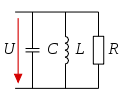
\includegraphics[scale=1]{a04/Parallelschw.png}\\
	\tiny{Abb.5: Parallelschwingkreis \cite{wmen}}
	\end{minipage}
	\begin{minipage}{0.4\textwidth}
	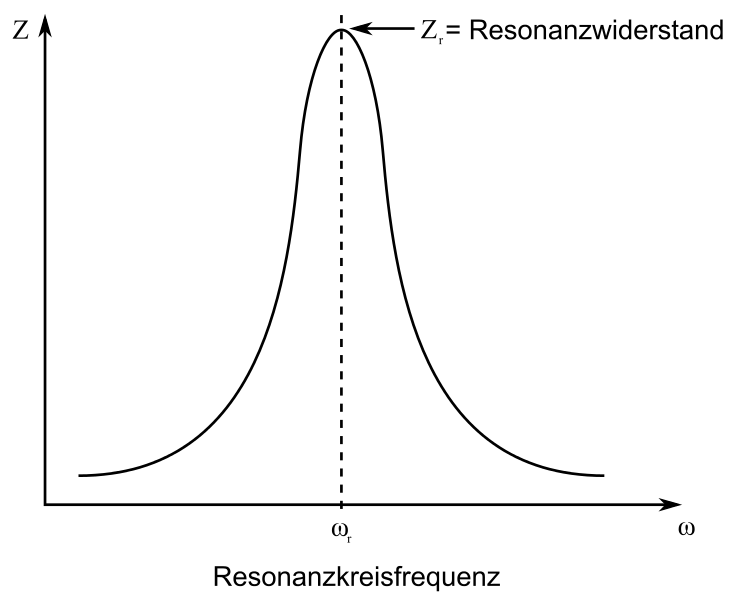
\includegraphics[scale=0.2]{a04/ParallelschwSig.png}\\
	\tiny{Abb.6: Resonanzwiderstand \cite{wmen}} 
	\end{minipage}
\end{center}
\begin{itemize}
	\item Der Parallelschwingkreis verhält sich genau entgegen gesetzt zum Reihenschwingkreis
	\item Dieser zeigt bei niedrigen und hohen Frequenzen das Verhalten eines Leiters
	\item Bei der Resonanzfrequenz hingegen steigt der Wellenwiderstand an, da hier nur noch der ohmsche Widerstand wirkt
\end{itemize}
\end{frame}

\subsection*{Resonanz\-frequenz}
\begin{frame}
  \frametitle{Resonanzfrequenz}
  \begin{block}{Resonanzfrequenz}
    Frequenz der äußeren Anregung, bei der die resultierende Amplitude maximal wird.
  \end{block}

  Das gilt, wenn der induktive Blindwiderstand $X_L$ gleich dem kapazitiven Blindwiderstand $X_C$ ist. Damit ergibt sich für die Resonanzfrequenz $f_0$:
  \begin{block}{Resonanzfrequenz}
    \begin{center}
      $f_0 = \cfrac{1}{2\pi \cdot \sqrt{L \cdot C}}$
    \end{center}
  \end{block}
\end{frame}

\begin{frame}
  \frametitle{Resonanzfrequenz}
  Herleitung:
  \begin{align*}
    X_L &= X_C \\
    \omega \cdot L &= \frac{1}{\omega \cdot C} & \text{mit } \omega = 2\pi \cdot f \\
    2\pi \cdot f \cdot L &= \frac{1}{2\pi \cdot f \cdot C} & \cdot\  2\pi \cdot f \\
    4\pi^2 \cdot f^2 \cdot L &= \frac{1}{C} & \div\  L \\  
    4\pi^2 \cdot f^2 &= \frac{1}{L \cdot C} & \sqrt{\ } \\
    2\pi \cdot f &= \frac{1}{\sqrt{L \cdot C}} & \div\  2\pi \\
    f &= \frac{1}{2\pi \cdot \sqrt{L \cdot C}}
  \end{align*}
\end{frame}


\begin{frame}
  \begin{tabular}{l||p{.8\textwidth}}\hline
    \textbf{TD207} & \textbf{Wie groß ist die Resonanzfrequenz dieser Schaltung, wenn $C_1 = 0,1nF$, $C_2 = 1,5nF$, $C_3 = 220pF$ und $L = 1mH$ beträgt?} \\
    & 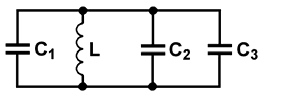
\includegraphics[width=.8\textwidth,height=.3\textheight,keepaspectratio]{a04/td207.png} \\ \hline\hline
    A & $1,18 kHz$ \\ \hline
    B \only<2>\checkmark & $117,973 kHz$ \\ \hline
    C & $1,17973 MHz$ \\ \hline
    D & $11,979 kHz$ \\ \hline
  \end{tabular}
\end{frame}

% -> siehe Aufgabenblatt
% \begin{frame}
%   \begin{tabular}{l||p{.8\textwidth}}\hline
%     \textbf{TD209} & \textbf{Welche Resonanzfrequenz $f_{res}$ hat die Parallelschaltung einer Spule von $2 \mu H$ mit einem Kondensator von $60 pF$ und einem Widerstand von $10 k\Omega$?} \\ \hline\hline
%     A & $145,288 kHz$ \\ \hline
%     B & $1,45288 MHz$ \\ \hline
%     C & $145,288 MHz$ \\ \hline
%     D \only<2>\checkmark & $14,5288 MHz$ \\ \hline
%   \end{tabular}
% \end{frame}



\subsection*{Bandbreite}
\begin{frame}
\frametitle{Bandbreite eines Schwingkreises}
\begin{center}
	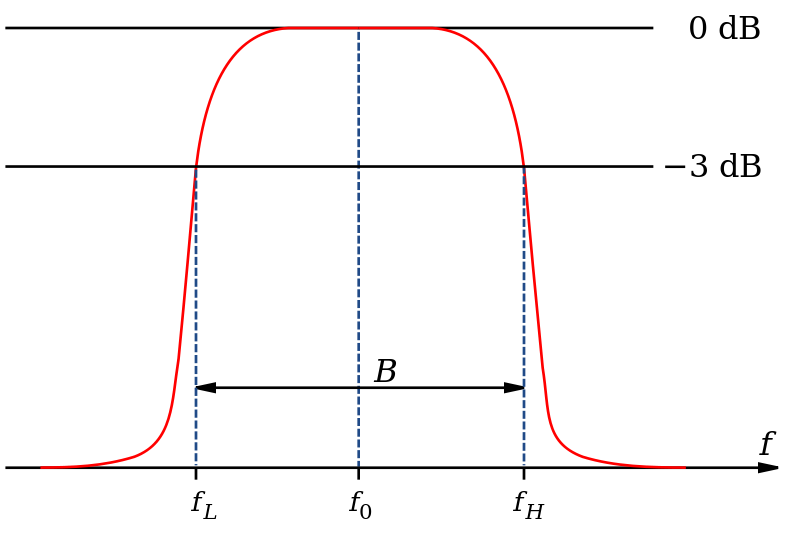
\includegraphics[scale=0.3]{a04/bandwidth.png}\\
	\tiny{Abb.7: Bandbreite \cite{wmen}}
\end{center}
Untere $f_L$ und obere Grenzfrequenz $f_H$ festgelegt beim $-3dB$-Punkt.
\end{frame}

\subsection*{Güte}

\begin{frame}
  \frametitle{Die Güte}
  \begin{itemize}
    \item Bandbreite hängt von der Güte des Schwingkreises ab
    \item Güte hängt vom (reellen) Widerstand der Spule $X_L$ ab
    \item Kondensatorverluste sind bei niedrigen und mittleren Frequenzen vernachlässigbar klein
  \end{itemize}
  \vspace{1em}
  \begin{block}{Reihenschwingkreis}
    \begin{center}
      $Q = \cfrac{X_L}{R_S}$
    \end{center}
  \end{block}
  \begin{block}{Parallelschwingkreis}
    \begin{center}
      $Q = \cfrac{R_P}{X_L}$
    \end{center}
  \end{block}
\end{frame}

\begin{frame}
  \frametitle{Die Güte}
  Kennt man die Güte und die Resonanzfrequenz $f_0$ eines Schwingkreises, so lässt sich die Bandbreite bestimmen:
  \begin{block}{Bandbreite}
    \begin{center}
      $B = \cfrac{f_0}{Q}$
    \end{center}
  \end{block}
  Und damit ergibt sich dieser Zusammenhang:
  \begin{block}{Güte}
    \begin{center}
      $Q = \cfrac{f_0}{B} = \cfrac{R_P}{X_L} = \cfrac{X_L}{R_S}$
    \end{center}
  \end{block}
\end{frame}

\begin{frame}
  \begin{tabular}{l||p{.8\textwidth}} \hline
    \textbf{TD214} & \textbf{Welchen Gütefaktor $Q$ hat die Reihenschaltung einer Spule von $100 \mu H$ mit einem Kondensator von $0,01 \mu F$ und einem Widerstand von $10 \Omega$?} \\ \hline\hline
    A & 1 \\ \hline
    B & 0,1 \\ \hline
    C \only<2>\checkmark & 10 \\ \hline
    D & 100 \\ \hline
  \end{tabular}
\end{frame}

\section*{Quarz}
\begin{frame}
  \frametitle{Der Quarz als Schwingkreis}
  \begin{center}
    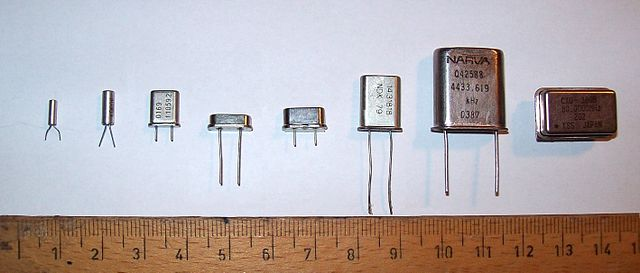
\includegraphics[width=\textwidth,height=.4\textheight,keepaspectratio]{a04/Quartz.jpg}\\
    {\tiny Abb.8: Verschiedene Bauformen von Quarzen}
  \end{center}
  \begin{itemize}
    \item Englisch: quar\textbf{t}z
    \item Besteht aus reinem Siliziumdioxid und wird aus einem Quarzkristall als dünnes Plättchen herausgeschnitten
    \item Verhalten ist durch den umgekehrten piezoelektrischen Effekt gekennzeichnet
    \item Ist ein Schwingkreis von hoher Güte und geringer Bandbreite
    \item Bessere Frequenzstabilität als LC-Oszillatoren
  \end{itemize}
\end{frame}

\begin{frame}
  \begin{tabular}{l||p{.8\textwidth}} \hline
    \textbf{TF412} & \textbf{Ein Frequenzmarken-Generator in einem Empfänger sollte möglichst}\\ \hline \hline
    A & ein BFO sein. \\ \hline
    B & ein RC-Oszillator sein. \\ \hline
    C \only<2>\checkmark & ein Quarzoszillator sein. \\ \hline
    D & ein LC-Oszillator sein. \\ \hline
  \end{tabular}
\end{frame}

\begin{frame}
  \begin{tabular}{l||p{.8\textwidth}} \hline
    \textbf{TD234} & \textbf{Ein Quarzfilter mit einer der \emph{(sic!)} 3-dB-Bandbreite von 500~Hz eignet sich besonders zur Verwendung in einem Sendeempfänger für} \\ \hline\hline
    A & SSB. \\ \hline
    B & FM. \\ \hline
    C & AM. \\ \hline
    D \only<2->\checkmark & CW. \\ \hline
  \end{tabular}

  \pause
  \vspace{2em}
  Die Frage gibt für alle Antwortmöglichkeiten, aber unterschiedlichen Bandbreiten:
  \begin{description}
    \item[2,3~kHz $\rightarrow$] \only<3>{SSB}
    \item[6~kHz $\rightarrow$] \only<3>{AM}
    \item[12~kHz $\rightarrow$] \only<3>{FM}
  \end{description}
\end{frame}

\section*{Filter}
\subsection*{Tiefpass}
\begin{frame}
\frametitle{Tiefpass}
\begin{center}
	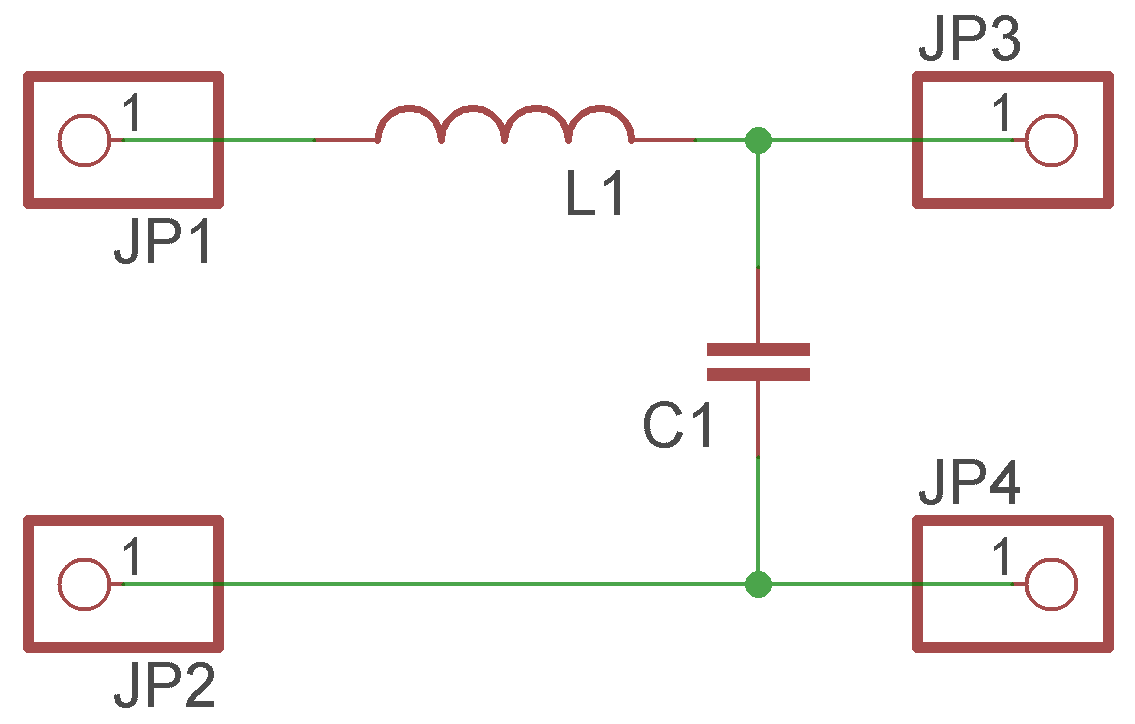
\includegraphics[width=\textwidth,height=.5\textheight,keepaspectratio]{e07/LC-Tiefpass.png}\\
	Abb.8: LC-Tiefpass
\end{center}
\begin{itemize}
	\item Bei steigender Frequenz sinkt der Blindwiderstand $X_L$ und der Blindwiderstand $X_C$ steigt
	\item Bei sinkender Frequenz hingegen steigt $X_L$ und $X_C$ sinkt
	\item Dadurch werden nur niedrige Frequenzen durchgelassen 
\end{itemize}
\end{frame}

\subsection*{Hochpass}
\begin{frame}
\frametitle{Hochpass}
\begin{center}
	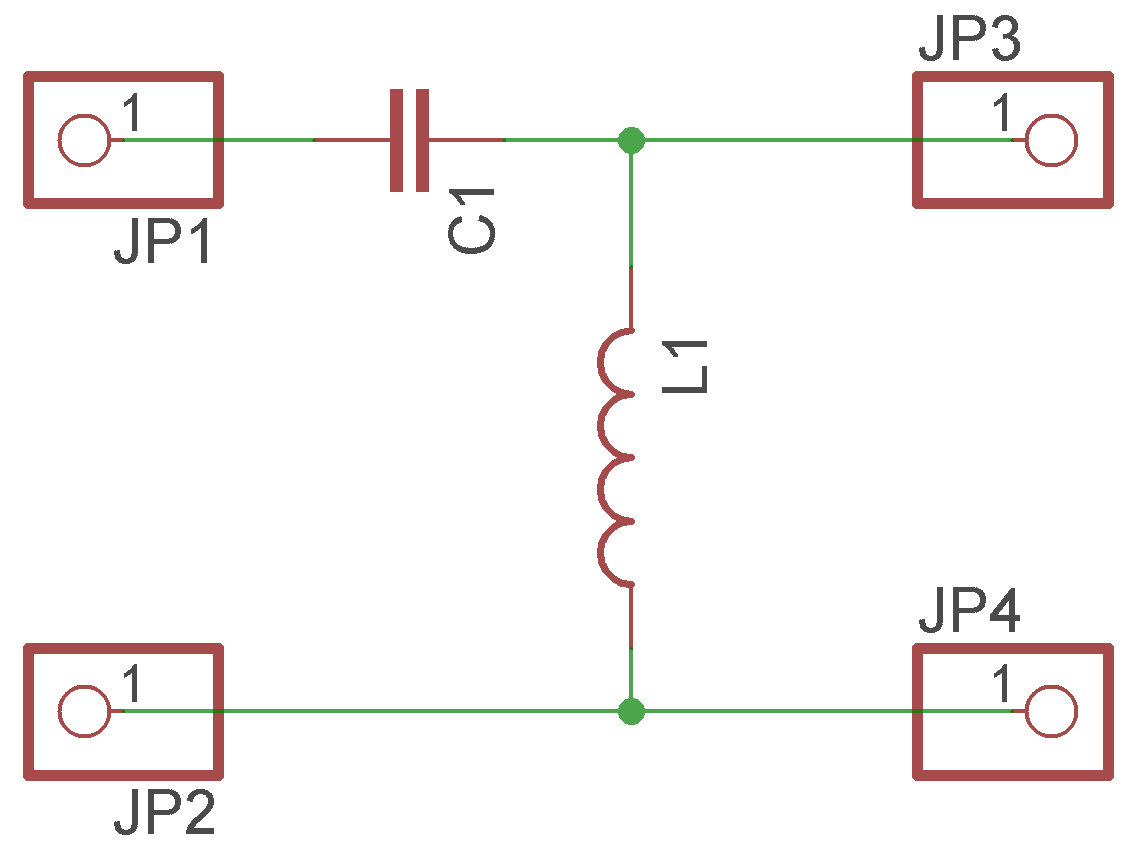
\includegraphics[width=\textwidth,height=.5\textheight,keepaspectratio]{e07/LC-Hochpass.png}\\
	Abb.9: LC-Hochpass
\end{center}
\begin{itemize}
	\item Bei steigender Frequenz steigt der Blindwiderstand $X_L$ und der Blindwiderstand $X_C$ sinkt
	\item Bei sinkender Frequenz hingegen sinkt $X_L$ und $X_C$ steigt
	\item Dadurch werden nur hohe Frequenzen durchgelassen 
\end{itemize}
\end{frame}

\subsection*{Bandpass}
\begin{frame}
  \frametitle{Bandpass}
  \begin{center}
    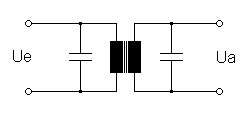
\includegraphics[width=\textwidth,height=.5\textheight,keepaspectratio]{a04/BandpassSpulen.png}\\
    Abb.12: Bandpass aus induktiv gekoppelten Schwingkreisen \cite{wpde}
  \end{center}
  \begin{itemize}
    \item Mehrere Parallelschwingkreise können zu Bandpässen gekoppelt werden
    \item Je nachdem wie fest\,/\,lose die Schwingkreise gekoppelt sind, ändert sich die Bandbreite des Bandpasses
  \end{itemize}
\end{frame}

\subsection*{Saugkreis}
\begin{frame}
  \frametitle{Saugkreis}
  \begin{center}
    % https://upload.wikimedia.org/wikipedia/commons/c/c9/Saugkreis.png
    \includegraphics<1>[width=\textwidth,height=.5\textheight,keepaspectratio]{e07/Saugkreis.png}
    \includegraphics<2>[width=\textwidth,height=.5\textheight,keepaspectratio]{e07/SerirenschwSig.png}
  \end{center}
  \pause
  \begin{itemize}
    \item vor und nach der Resonanzfrequenz hoher Widerstand
    \item nur Wechselspannungen mit Frequenzen in der Nähe der Resonanzfrequenz werden durchgelassen
    \item Anwendung: Audiotechnik
  \end{itemize}
\end{frame}

\subsection*{Sperrkreis}
\begin{frame}
  \frametitle{Sperrkreis}
  \begin{center}
    % https://upload.wikimedia.org/wikipedia/commons/e/ef/Sperrkreis.png
    \includegraphics<1>[width=\textwidth,height=.5\textheight,keepaspectratio]{e07/Sperrkreis.png}
    \includegraphics<2>[width=\textwidth,height=.5\textheight,keepaspectratio]{e07/ParallelschwSig.png}
  \end{center}
  \pause
  \begin{itemize}
    \item bei der Resonanzfrequenz hoher Widerstand
    \item die Resonanzfrequenz wird blockiert
    \item Anwendungen: Mehrbandantennen; Filtern von starken Sendern
  \end{itemize}
\end{frame}

\subsection*{Resonanz\-trans\-formation}
\begin{frame}
  \frametitle{Resonanztransformation}
  \begin{center}
    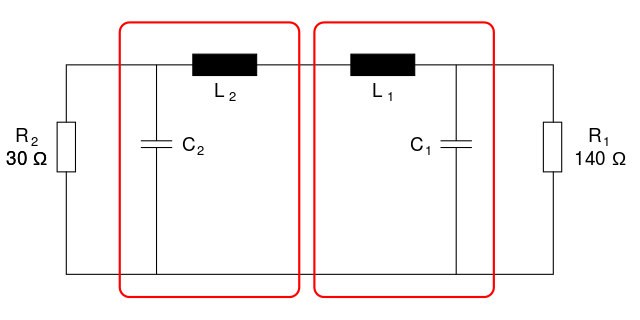
\includegraphics[scale=0.2]{a04/Pi-Filter.png}\\
    Abb.13: Pi- oder auch Collinsfilter \cite{wpde}
  \end{center}
  \begin{itemize}
    \item Schwingkreise in Resonanz eignen sich gut zum Anpassen von Impedanzen
    \item Nicht die Induktivität, sondern die Kapazitäten sind für die Anpassung verantwortlich
    \item Oft werden Drehkondensatoren benutzt, um stufenlos anpassen zu können
    \item Eingesetzt in Tunern oder Verstärkern (mit den zwei Drehkondensatoren \emph{Load} und \emph{Plate}).
  \end{itemize}
\end{frame}

\begin{frame}
  \begin{columns}
    \column{.65\textwidth}
    \begin{tabular}{l||p{.8\textwidth}} \hline
      \textbf{TD230} & \textbf{Das folgende Bild zeigt ein typisches ZF-Filter und vier seiner möglichen Übertragungskurven (a bis d). Welche Kurve ergibt sich bei kritischer Kopplung und welche bei überkritischer Kopplung?} \\ \hline\hline
      A \only<2>\checkmark & Die b-Kurve zeigt kritische, die a-Kurve zeigt überkritische Kopplung. \\ \hline
      B & Die a-Kurve zeigt kritische, die b-Kurve zeigt überkritische Kopplung. \\ \hline
      C & Die c-Kurve zeigt kritische, die b-Kurve zeigt überkritische Kopplung. \\ \hline
      D & Die d-Kurve zeigt kritische, die c-Kurve zeigt überkritische Kopplung. \\ \hline
    \end{tabular}
    \column{.3\textwidth}
      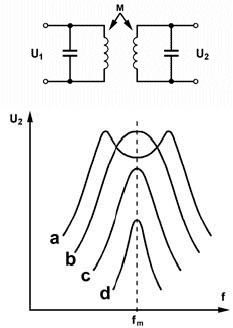
\includegraphics[width=\textwidth,height=.95\textheight,keepaspectratio]{a04/td230.png}
  \end{columns}
\end{frame}


\renewcommand{\refname}{Referenzen}

\hypertarget{refs}{}
\textcolor{white}{} \\ %\vspace{} geht nicht
\Large Referenzen/Links
\footnotesize

\begin{thebibliography}{}
    \bibitem{a04}   Moltrecht A 04: \\
                    \url{http://www.darc.de/referate/ajw/ausbildung/darc-online-lehrgang/technik-klasse-a/technik-a04/}
    
    \bibitem{wpde}    Wikipedia DE: \\
                    \url{http://de.wikipedia.org/wiki/lektrische_Energie#Elektrische_Energie_in_einem_elektrischen_Feld}\\ 
                    \url{http://de.wikipedia.org/wiki/Datei:Verschiedene_Schwingquarze.jpg}\\
                    \url{http://de.wikipedia.org/wiki/Datei:Schwingquarz-Ersatzschaltbild.png}\\
                    \url{http://de.wikipedia.org/wiki/Datei:BandpassSpulen.png}\\
    				\url{http://de.wikipedia.org/wiki/Datei:ResoTrafo_3.svg}\\
    				
    \bibitem{wpen}	Wikipedia EN:\\
    				\url{http://en.wikipedia.org/wiki/File:Tuned_circuit_animation_3.gif}\\
    				
    \bibitem{wmde}	Wikimedia DE:\\
    				\url{http://commons.wikimedia.org/wiki/File:LC_circuit_4_times_new_version.svg?uselang=de}\\
   \vspace{1cm}
   \bibitem{wmen}	Wikimedia EN:\\
   					\url{http://commons.wikimedia.org/wiki/File:RLC_series_circuit_v1.svg}\\
   					\url{http://commons.wikimedia.org/wiki/File:Resonanzwiderstand_serie.svg}\\
   					\url{http://commons.wikimedia.org/wiki/File:KondiSpuleWiderstandParallel.svg}\\
   					\url{http://commons.wikimedia.org/wiki/File:Resonanzwiderstand_parallel.svg}\\
   				  					
\end{thebibliography} 

% Hier könnte noch eine Kontaktfolie stehen

\end{document}

